% Prepared by Calvin Kent
%
% Assignment Template v19.02
%
%%% 20xx0x/MATHxxx/Crowdmark/Ax
%
\documentclass[12pt]{article} %
\usepackage{CKpreamble}
\usepackage{CKassignment}
\usepackage{tkz-euclide}
\usepackage{physunits}
\usepackage{physics}
\usepackage{lmodern}
\usepackage{microtype}
\usepackage{upgreek}
\usepackage[misc]{ifsym}

%%% Maths and science packages

\usepackage{amsmath,amsthm,amssymb}
\usepackage{pgfplots}
	\usetikzlibrary{
		calc,
		patterns,
		positioning
	}
	\pgfplotsset{
		compat=1.16,
		samples=200,
		clip=false,
		my axis style/.style={
			axis x line=middle,
			axis y line=middle,
			legend pos=outer north east,
			axis line style={
				->,
			},
			legend style={
				font=\footnotesize
			},
			label style={
				font=\footnotesize
			},
			tick label style={
				font=\footnotesize
			},
			xlabel style={
				at={
					(ticklabel* cs:1)
				},
				anchor=west,
				font=\footnotesize,
			},
			ylabel style={
				at={
					(ticklabel* cs:1)
				},
				anchor=west,
				font=\footnotesize,
			},
			xlabel= $t$,
			ylabel=$\vec d (\m \tx{[East]})$
		},
	}
	\tikzset{
		>=stealth
	}

%%% Tables and figures packages

\usepackage{float}
\usepackage{caption}
	\captionsetup{
		format=plain,
		labelfont=bf,
		font=small,
		justification=centering
	}
	
%%% Numbers and sets

\newcommand{\E}{\mathrm{e}}

\newcommand{\tx}[1]{\text{#1}}

\begin{document}
    \pagenumbering{arabic}
    % Start of class settings ...
    \renewcommand*{\coursecode}{Physics Homework} % renew course code
    \renewcommand*{\assgnnumber}{4} % renew assignment number
    \renewcommand*{\submdate}{August 26, 2021} % renew the date
    \renewcommand*{\studentfname}{Abdullah} % Student first name
    \renewcommand*{\studentlname}{Zubair} % Student last name
    %\renewcommand*{\studentnum}{SNumber} % Student number

    \renewcommand\qedsymbol{$\blacksquare$}
    \setfigpath
    % End of class settings 
    \pagestyle{crowdmark}
    \newgeometry{left=18mm, right=18mm, top=22mm, bottom=22mm} % page is set to default values
    \fancyhfoffset[L,O]{0pt} % header orientation fixed
    % End of class settings
    %%% Note to user:
    % CTRL + F <CHANGE ME:> (without the angular brackets) in CKpreamble to specify graphics paths accordingly.
    % The command \circled[]{} accepts one optional and one mandatory argument.
    % Optional argument is for the size of the circle and mandatory argument is for its contents.
    % \circled{A} produces circled A, with size drawn for letter A. \circled[TT]{A} produces circled A with size drawn for TT.
    % https://github.com/CalvinKent/My-LaTeX
    %%%
    % Crowdmark assignment start


    %%%%%%%%%%%%%%%%%%%%%%%%%%%%%%%%%%%%%%%%%%%%%%%%%%%%%%%%%%%%%%%%%%%%%%%%%%%%%%%%%%%%%%%%%%%%%%%%%%%%%%%%
    %%%%%%%%%%%%%%%%%                  PROBLEM IDEAS                  %%%%%%%%%%%%%%%%%%%%%%%%%%%%%%%%%%%%%%
    %%%%%                   ----------------------------------------                                %%%%%%%%

    % --> Do a hard tangent line problem







\begin{qstn}[1] % qnumber, qname, qpoints
    Answer the following True/False questions (\textbf{Assume [East] is positive})
    \begin{enumerate}
        \item An object under uniform motion has a
            \begin{enumerate}[label = (\alph*)]
                \item Non-zero average acceleration in the positive direction (T / F) 
                \item Zero average acceleration (T / F)
            \end{enumerate}
        \item De-acceleration is just acceleration in the same direction of motion (T / F)
        \item Suppose that a bullet accelerates at $\vec a_{av} = +1.068 \km / \s^2$ from rest to a final velocity of $\vec v_f = +356 \m / \s$. Then,
            \begin{enumerate}[label = (\alph*)]
                \item The time elapsed was $\Delta t = 3\s$
                \item If I double the acceleration of the bullet, then $\Delta t$ doubles as well. (T / F)
            \end{enumerate}
        \item Suppose a Velocity V. Time plot is represented by $y = 2x + 4$,
            \begin{enumerate}[label = (\alph*)]
                \item The average acceleration is uniform (T / F)
                \item The initial velocity of the body at $t = 0$ was $\vec v_i = +4 \m / \s$ (T / F)
                \item The displacement over the time interval $[0,2]$ was $\Delta \vec d = +12\m$ (T / F)
                \item The average acceleration is $\vec a_{av} = +2\m / \s^2$ (T / F)
            \end{enumerate}
        \item A secant line on a Velocity V. Time graph over the interval $[t_1,t_2]$ gives me the instantaneous acceleration over the time interval $[t_1,t_2]$. (T / F)
        \item Suppose a Position V. Time plot is represented by $y = x^2 + 4$. Then,
            \begin{enumerate}[label = (\alph*)]
                \item The object is slowing down in the positive direction. (T / F)
                \item The object is experiencing uniform motion. (T / F)
                \item The object \emph{may} be experiencing uniform acceleration (T / F).
                \item The initial position vector of the object at $t = 0$ is $\vec d_i = 2 \m$
            \end{enumerate}
        \item Suppose that the tangent line to a Position V. Time plot at $t = 4$ was represented by the equation $y = -3x + 7$. Then,
            \begin{enumerate}[label = (\alph*)]
                \item The instantaneous velocity of the object at $t = 4$ was $\vec v = +3 \m / \s$
                \item The instantaneous velocity of the object at $t = 5$ was $\vec v = -3 \m / \s$
                \item Suppose that the Velocity V. Time plot for the object happened to be linear, then the average velocity of the object must have been $\vec v_{av} = -3\m / \s$. (T / F)
            \end{enumerate}
        \item Suppose a Velocity V. Time plot is represented by $y = -x + 3$, then the displacement over the time interval $[0,8]$ is $\Delta \vec d = +0 \m$. (T / F)
        \item Suppose that the average acceleration of an object in motion differs at two distinct points in time, then the Velocity V. Time graph must have been linear. (T / F)

    \end{enumerate}

 \end{qstn}

 \begin{qstn}[2]
    Answer the following multiple choice questions.
    \begin{enumerate}
        \item Which of the following statements are correct about the plot below? (Assume that the motion lasted for $4$ seconds)
    \begin{center}
        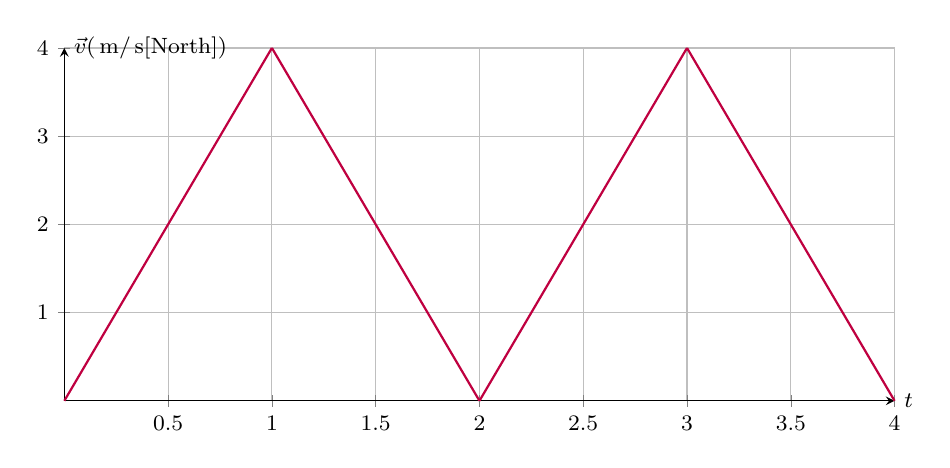
\begin{tikzpicture}
        \begin{axis}[
            my axis style,
            width=\textwidth,
            height=.5\textwidth,
            ylabel=$\vec v (\m / \s \tx{[North]})$,
            grid
        ]
        
        \addplot[
            domain=0:1,
            thick,
            purple,
            -
        ]
        {4*x};
    
        \addplot[
            domain=1:2,
            thick,
            purple,
            -
        ]
        {-4*x + 8};

        \addplot[
            domain=2:3,
            thick,
            purple,
            -
        ]
        {4*x - 8};
    
        \addplot[
            domain=3:4,
            thick,
            purple,
            -
        ]
        {-4*x + 16};
        
        \fill[
            black
        ];
        
        \end{axis}
        \end{tikzpicture}
    \end{center}
    
    
            \begin{enumerate}[label = (\alph*)]
                \item The body experienced uniform acceleration throughout the entire trip.
                \item Within the time interval $[0,2]$ the average acceleration was $\vec a_{av} = +0 \m / \s^2$
                \item Within the time interval $[3,4]$ the average acceleration was $\vec a_{av} = -4 \m / \s^2$
                \item Within the time interval $[1,4]$ the average acceleration was $\vec a_{av} = -1.333 \m / \s^2$
                \item At $t = 2\s$, the instantaneous acceleration was $\vec a_{av} = +4 \m / \s^2$
                \item At $t = 3.4\s$, the instantaneous acceleration was $\vec a_{av} = -4 \m / \s^2$
                \item The average acceleration is \emph{not} the same as the instantaneous acceleration for each point in time.
            \end{enumerate}

        \item The Velocity V. Time plot for a body in motion is similar to $y = 4x + 7$.
            \begin{enumerate}[label = (\alph*)]
                \item The displacement over the first $t = 4\s$ was $\Delta \vec d = +23\m$.
                \item The object experienced uniform motion.
                \item The object experienced uniform acceleration.
                \item The object was speeding up in the positive direction
            \end{enumerate}
        
        \end{enumerate}

    \end{qstn}

    \begin{qstn}[3]
        Answer the following inquires about the plot below,
        

        \begin{center}
            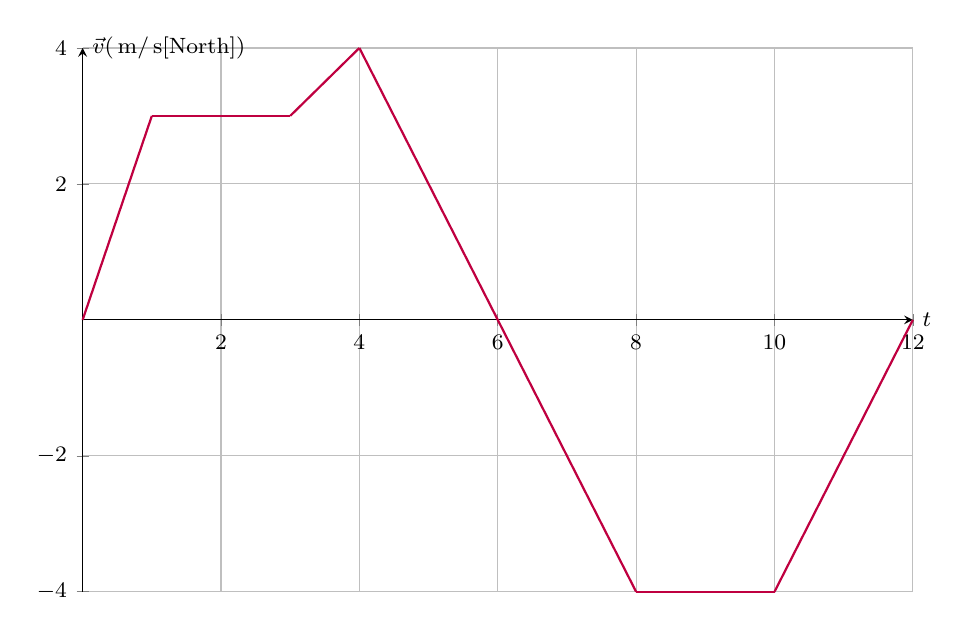
\begin{tikzpicture}
            \begin{axis}[
                my axis style,
                width=\textwidth,
                height=.7\textwidth,
                ylabel=$\vec v (\m / \s \tx{[North]})$,
                grid
            ]
            
            \addplot[
                domain=0:1,
                thick,
                purple,
                -
            ]
            {3*x};
        
            \addplot[
                domain=1:3,
                thick,
                purple,
                -
            ]
            {3};
    
            \addplot[
                domain=3:4,
                thick,
                purple,
                -
            ]
            {x};
        
            \addplot[
                domain=4:8,
                thick,
                purple,
                -
            ]
            {-2*x + 12};

            \addplot[
                domain=8:10,
                thick,
                purple,
                -
            ]
            {-4};

            \addplot[
                domain=10 : 12,
                thick,
                purple,
                -
            ]
            {2*x - 24};
            
            \fill[
                black
            ];
            
            \end{axis}
            \end{tikzpicture}
        \end{center}

        \begin{enumerate}[label = (\alph*)]
            \item The displacement over the time interval $[1,3]$.
            \item The displacement over the time interval $[3,8]$.
            \item The displacement by the end of the trip ($\Delta t = 12\s$)
        \end{enumerate}


 \end{qstn}

\begin{qstn}[4]
    Answer the following inquires about the Velocity V. Time plot below,
    \begin{center}
        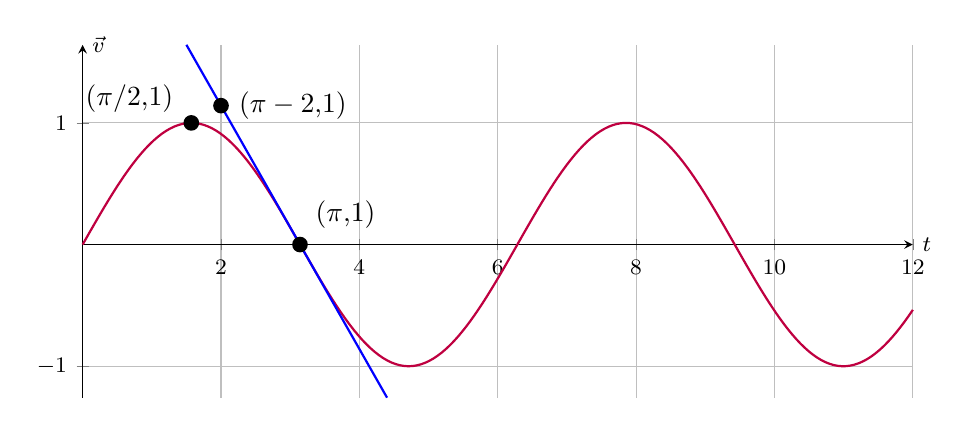
\begin{tikzpicture}
        \begin{axis}[
            my axis style,
            width=\textwidth,
            height=.5\textwidth,
            ylabel=$\vec v$,
            grid
        ]
        
        \addplot[
            domain=0:12,
            thick,
            purple,
            -
        ]
        {sin(deg(x))};

        \addplot[
            domain=1.5:4.4,
            thick,
            blue,
            -
        ]
        {-1*x + 3.141592689};

        \fill[
            black
        ];

        \node[label={45:{($\pi$,1)}},circle,fill,inner sep=2pt] at (axis cs:3.141592689,0) {};
        \node[label={175:{($\pi / 2$,1)}},circle,fill,inner sep=2pt] at (axis cs:1.570796,1) {};
        \node[label={0:{($\pi - 2$,1)}},circle,fill,inner sep=2pt] at (axis cs:2,1.1415926) {};
        
        \end{axis}
        \end{tikzpicture}
    \end{center}

    \begin{enumerate}[label = (\alph*)]
        \item Determine the average acceleration within the time interval $[\pi / 2,\pi]$.
        \item Determine the instantaneous acceleration at time $t = \pi$.\\
        (\textbf{Hint:} The line in blue is a tangent line to the plot at $t = \pi$)
        \item Prove that $\vec a_{av} = +0\m / \s^2$ over the interval $[0,\pi]$.


    \end{enumerate}


 \end{qstn}

 \begin{qstn}[5]
    Given the Position V. Time plot below, answer the following inquires.
    \begin{center}
        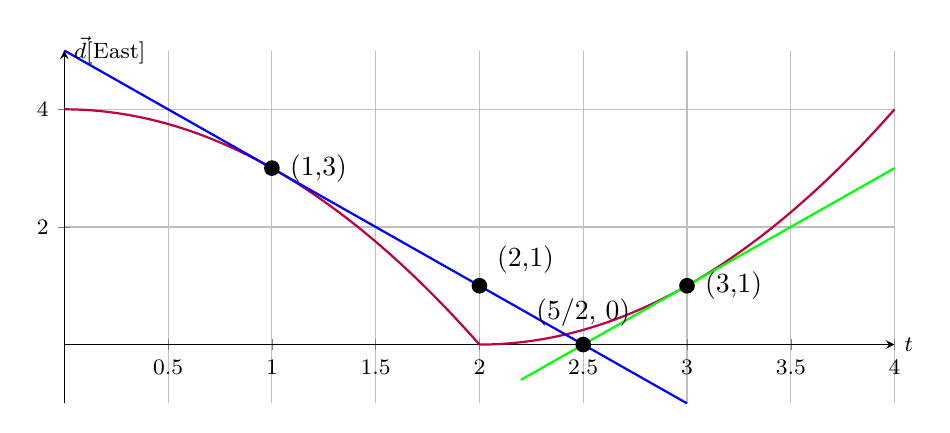
\begin{tikzpicture}
        \begin{axis}[
            my axis style,
            width=\textwidth,
            height=.5\textwidth,
            ylabel=$\vec d \tx{[East]}$,
            grid
        ]
        
        \addplot[
            domain=0:2,
            thick,
            purple,
            -
        ]
        {-1*x*x + 4};

        \addplot[
            domain=2:4,
            thick,
            purple,
            -
        ]
        {(x-2)*(x-2)};

        \addplot[
            domain=0:3,
            thick,
            blue,
            -
        ]
        {-2*x + 5};

        \addplot[
            domain=2.2:4,
            thick,
            green,
            -
        ]
        {2*x - 5};

        \fill[
            black
        ];

        \node[label={20:{(2,1)}},circle,fill,inner sep=2pt] at (axis cs:2,1) {};
        \node[label={0:{(1,3)}},circle,fill,inner sep=2pt] at (axis cs:1,3) {};
        \node[label={0:{(3,1)}},circle,fill,inner sep=2pt] at (axis cs:3,1) {}; 
        \node[label={90:{(5/2, 0)}},circle,fill,inner sep=2pt] at (axis cs:2.5,0) {}; 
        
        \end{axis}
        \end{tikzpicture}
    \end{center}

    \begin{enumerate}[label = (\alph*)]
        \item Determine the average velocity over the time interval $[0,2]$.
        \item Describe the motion over the time interval $[0,2]$
        \item Determine the instantaneous velocity at $t = 1$.\\
        (\textbf{Hint:} The line in blue is a tangent line to the plot at $t = 2$)
        \item Describe the motion of the plot after $t = 2$ seconds.
        \item The slope of the tangent line in green is $m = +12$. Determine the equation of the line ($y = mx + b$).
    \end{enumerate}

 \end{qstn}

\begin{qstn}[6]
 A ball is kicked with an initial velocity of $\vec v_i = 80 \m / \s \tx{[South]}$. It experiences a drag force and de-accelerates at $\vec a_{av} = 5 \m / \s^2 \tx{[North]}$.
            \begin{enumerate}[label = (\alph*)]
                \item Determine the final velocity of the ball after $\Delta t = 40\s$
                \item At what time $t$ did ball start to travel in the Northward direction.
            \end{enumerate}
\end{qstn}
        

 \begin{qstn}[7]
    Patrick has decided to embark on a journey throughout the sea on a boat. The boat has a relative velocity of $\vec v_{PG} = 400 \m / \s\tx{[East]}$ relative to the ground (G). On the boat, Patrick is walking with a relative velocity of $\vec v_{PB} = +50 \m / \s$ relative to the boat. Determine the average acceleration of patrick relative to the ground. Determine,
    \begin{enumerate}[label = (\alph*)]
        \item The velocity of patrick relative to the ground ($\vec v_{PG}$)\\
        (\textbf{Hint: }Use the exact same technique from when we were working with position vectors, i.e $\vec v_{AC} = \vec v_{AB} + \vec v_{BC}$)
        \item The average acceleration of Patrick relative to the ground over a time period of $\Delta t = 40\s$ if everything was \emph{initially} at rest.

    \end{enumerate}

 \end{qstn}




\begin{qstn}[8]
    A car is initially traveling at an initial velocity $\vec v_i = 412 \m / \s$[\tx{East}]. The car then de-accelerates at an average acceleration of $\vec a_{av}$ to come to a rest at a red light over a duration of $\Delta t$. When the light turns green, the car accelerates at an average acceleration $-\vec a_{av}$ over a time period $2\Delta t$, to reach a final velocity of $\vec v_f = 240 \m / \s$ \tx{[East]} . Determine the the average acceleration $\vec a_{av}$. \\(\textbf{Hint :} Setup the correct equations to get rid of $\Delta t$) 
 \end{qstn}






\end{document}









